
\section{Mind Wandering}
\label{sec: mind_wandering}
Mind wandering, frequently conceptualized as "task-unrelated thinking," encompasses thoughts not directly related to the task at hand \cite{Barron2011} \cite{McVay2009}. However, Smallwood and Schooler\cite{SmallwoodSchooler2015} contend that this definition is overly broad as it includes internally generated thoughts and those stimulated by external environmental cues such as sounds or visuals. In "The Restless Mind," Smallwood and Schooler propose that mind wandering occurs when executive control transitions from focusing on a primary task to engaging with personally relevant goals. They outline three core consequences of this shift: First, tasks requiring extensive controlled processing consume significant working-memory resources, reducing mind wandering due to resource limitations. Second, mind-wandering episodes may impair the processing accuracy of external stimuli as cognitive resources are redirected toward internal tasks. Third, if a hierarchical model of goals is assumed, goal-related processes may be activated automatically, allowing a secondary personal goal to supersede the primary task focus.

Empirical evidence suggests that mind wandering frequency diminishes with an increase in the rate of stimulus presentation \cite{Antrobus1968} \cite{Giambra1995} \cite{Smallwood2004}, aligning with the first outcome posited by Smallwood and Schooler. This relationship implies that the stimulus presentation rate is critical when compiling a balanced dataset for research purposes. The studies by Antrobus\cite{Antrobus1968}, Giambra\cite{Giambra1995}, and Smallwood and Davies\cite{Smallwood2004} also indicate that mind wandering increases during well-practiced tasks, suggesting that repeated experimental runs can influence the distribution of mind wandering episodes. The hypothesis that mind wandering competes for working memory resources suggests task performance will likely deteriorate during mind-wandering episodes in sufficiently resource-demanding tasks. Teasdale and Dritschel\cite{Teasdale1995} demonstrated this effect in a random-number generation task, thereby confirming that task performance can indicate mind-wandering episodes and, consequently, work as part of a method for validating experimental labels.

\section{Detection of Mindwandering}

Detection of mind wandering presents significant challenges. As noted by Smallwood and Schooler \cite{SmallwoodSchooler2015}: 
"... at least three conceptual issues arise in the investigation of mind wandering: (a) the lack of direct experimental control, (b) the covert nature of self-generated thoughts, and (c) the validity and potential reactivity of introspective evidence."

\subsection{Verbal Reporting}
Verbal self-reporting serves as a rudimentary method for detecting mind wandering. Nevertheless, the reliability of self-reports is questionable. Schooler and Schreiber have shown that self-report accuracy can be assessed by correlating them with physiological markers, providing a more comprehensive understanding of their validity\cite{Schooler2004}.

\subsection{Thought Sampling}
Thought sampling includes two primary methods: self-caught and probe-caught. In self-caught mind wandering, individuals report mind wandering upon self-recognition; hence, the measurement focuses primarily on their awareness of mind-wandering rather than the underlying frequency episodes. Conversely, probe-caught mind wandering employs a method where subjects are intermittently questioned about their current mental state during the task. Responses may be self-classified by the subjects or experimenter-classified based on predefined criteria. Probe-caught sampling thus leads to a better estimate of the actual mind-wandering frequency. However, self-classification may lead to an artificially high reporting rate of mind wandering due to increased vigilance following instructions about mind wandering characteristics \cite{Giambra1995}. It is also crucial to recognize that self-awareness might still be a limiting factor, as participants may not fully perceive their mental state, even when prompted. Despite this, self-classification offers practical advantages, such as reduced need for disclosing personal information and simplicity in self-assessment. \cite{SmallwoodSchooler2006}.

\subsection{Study design}
\label{subsec: study_design}
As previously discussed, accurately labeling mind-wandering episodes is fraught with difficulties. To enhance estimates' validity regarding individuals' true internal state, a triangulation method has been proposed \cite{SmallwoodSchooler2015}. This approach integrates self-classified and probe-caught mind-wandering reports with task performance metrics and neurophysiological data. This multidimensional strategy seeks to corroborate subjective reports through objective measures and scientific knowledge from earlier studies, thereby providing a more robust and reliable estimate of mind wandering.

The Sustained Attention to Response Task (SART) is a tool that has proven itself as robust in studying mind wandering through its ability to induce and measure lapses in attention during monotonous tasks\cite{Robertson1997}. The dual approach of combining real-time subjective experience sampling with objective performance measures, such as intra-individual reaction time variability, offers a comprehensive method to assess mind wandering accurately. This variability has been shown to predict mind wandering \cite{Baird2012}\cite{BastianSackur2013}, and such fits with the triangulation approach. 

By embedding experience-sampling probes into the SART,  datasets can be created with annotations of mind-wandering instances and subsequently validated by measurable performance metrics. The SART might be particularly suitable for settings where sustained attention is crucial and has been tested in different meditation studies using Vipassana\cite{Zanesco2013} and Mindfulness Training \cite{Morrison2014}. To further increase the validity of the labels collected, EEG Event-Related Potential (ERP) analysis has been used for SART validation\cite{Kam2011}. Thus, SART-generated data is likely to enhance the viability of datasets for predictive models in an EEG data contemplative research context, especially when validated through triangulation. 

\section{EEG Signals}
Electroencephalography, or EEG, is a method for measuring the brain's electrical activity. EEG is a non-invasive method where a set amount of electrodes are fitted to the subject's scalp in a predefined pattern, often a subset of the 10-10 system described in \autoref{fig: eeg_1010}. The electrode designs are split into dry and wet electrodes, where dry electrodes try to connect to the scalp itself. In contrast, wet electrodes use an electrically conductive gel to pass the signal from the scalp to the electrode. Each electrode, often called a channel, records a time series of electrical potentials, resulting in a data array of the number of channels times the length of the channel's time series ([n\_channel, time\_series\_lenght]). Thus, EEG recordings give a wave-like pattern over all channels, often visualized as in \autoref{fig: eeg_viz}.

\begin{figure}
    \centering
    \includegraphics[width=0.6\linewidth]{Figures/eeg/EEG_10-10_system_with_additional_information.png}
    \caption{EEG 10-10 System. Picture from \cite{Wiki1020EEG}.}
    \label{fig: eeg_1010}
\end{figure}
\begin{figure}
    \centering
    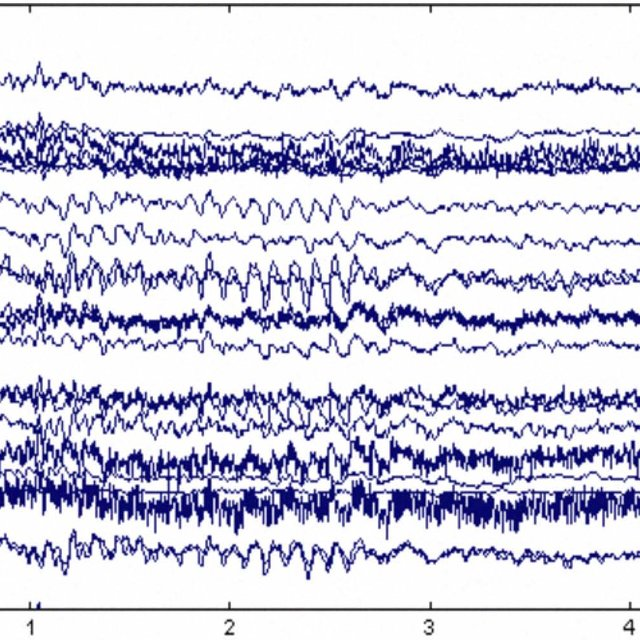
\includegraphics[width=0.6\linewidth]{Figures/eeg/eeg.jpg}
    \caption{Visualized EEG recording over several channels.}
    \label{fig: eeg_viz}
\end{figure}

\subsection{Waves}
The study of waves has a long history in the mathematical sciences, garnering interest from the likes of Newton, Maxwell, and Fourier. Fourier's seminal insight proved that any function could be represented as a series of simple sine waves. Conversely, complex waveforms can also be decomposed into these fundamental sine components, allowing the analysis of wave signals in their simplest forms\cite{bracewell1986fourier}.

\subsubsection{Empirical Mode Decompositions (EMD)}
Among the techniques for wave analysis, the Hilbert-Huang Transform (HHT)\cite{Huang1998EMD} stands out, particularly in comparison to the traditional Fourier Transform. The HHT is designed to decompose a signal into Intrinsic Mode Functions (IMFs). These IMFs are similar to the sine wave components in Fourier analysis but are specifically tailored for analyzing non-stationary signals whose statistical properties vary over time\cite{Huang1998EMD} .

A stationary process in stochastic terms is defined by statistical properties unchanging in time, such as consistent mean and variance, mathematically represented as \(F(x)\). In contrast, a non-stationary process exhibits time-dependent statistical properties, represented as \(F(x,t)\). Non-stationary signals, therefore, have a generator function that varies over time. Although all real-world signals are non-stationary to some degree, the rate of change often dictates their practical analysis\cite{Brockwell1991}. For instance, while the Moon's orbit exhibits minimal daily changes, making it practically stationary for short-term predictions, modeling its trajectory over millennia with today's parameters would yield significant inaccuracies. Contrary to the Moon's orbit, EEG signals of the brain exhibit rapid changes in the underlying generator functions, making their non-stationarity significant\cite{Klonowski2009}. 
 

\subsection{Multivariate Empirical Mode Decomposition}

The Multivariate Empirical Mode Decomposition (MEMD) represents a significant advancement in signal processing, particularly tailored for analyzing complex multidimensional signals\cite{Mandic2013}. This algorithm is an extension of the classical one-dimensional Empirical Mode Decomposition (EMD)\cite{Huang1998EMD}, designed to address the limitations of applying EMD separately to each channel of multidimensional data. Unlike the conventional approach, MEMD considers the interconnectedness of data channels, which is crucial for accurately interpreting signal information.

A practical illustration of MEMD's necessity can be observed in neuroscientific applications, such as analyzing neural signals captured by several electrodes over a cluster of neurons. Signals recorded from such clusters are influenced by both the spatial arrangement of the electrodes and the varying conductive properties of the intervening biological tissues. As a result, each electrode captures a signal that, while unique in timing and amplitude due to the distance and tissue permeability from the neural source, is fundamentally linked to the same originating neural event. The traditional EMD, if applied individually to each signal channel, would fail to capture these interdependencies, potentially leading to misleading conclusions about the neural activity.

MEMD, therefore, provides a more holistic view of multidimensional data by recognizing and preserving the intrinsic relationships among the channels. This makes it indispensable for accurately decomposing complex signals into their constituent IMFs.

\section{Introduction to Machine Learning}

Machine learning is a substantial field within computer science, which is distinguished by teaching computers the ability to learn from and make decisions based on data\cite{Mohammed2016}. This thesis will concentrate on the specific aspects of machine learning crucial for understanding the project's framework and the rationale behind critical decisions.

\subsection{Differentiating Machine Learning from Traditional Programming}

Traditional programming involves the creation of explicit, rule-based algorithms that instruct the computer on solving specific types of problems. This method is highly effective for a range of applications; however, it encounters limitations when the complexity of the problems increases, such as when rules must scale significantly\cite{Mohammed2016}. For instance, consider the challenge of identifying the number of fingers displayed in an image or classifying handwritten digits from the MNIST dataset\cite{deng2012mnist}. As illustrated in \autoref{fig: mnist2}, handwritten digits like the number "2" can vary significantly in shape and style, posing a substantial challenge for rule-based systems.

\begin{figure}
    \centering
    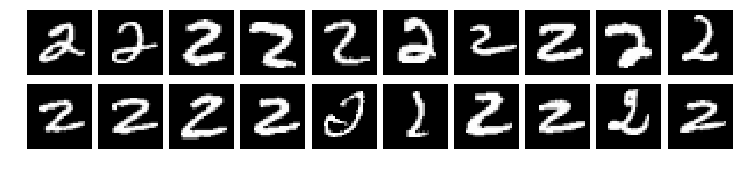
\includegraphics[width=250px]{Figures/MLintro/mnist2.png}
    \caption{Variations of the handwritten digit '2' from the MNIST dataset}
    \label{fig: mnist2}
\end{figure}

Humans can typically recognize these variations effortlessly, suggesting that a different approach is feasible for machines. This approach involves features, a distinct and recognizable element of the input data that forms a complete picture when combined with other features. Features can be engineered manually but can also be learned automatically from data, a foundational machine learning principle. As depicted in \autoref{fig: fromProgrammingToML}, the difference between traditional programming and machine learning involves shifting from manually coded instructions to systems that learn from data to identify and utilize features\cite{Mohammed2016}.

\begin{figure}
    \centering
    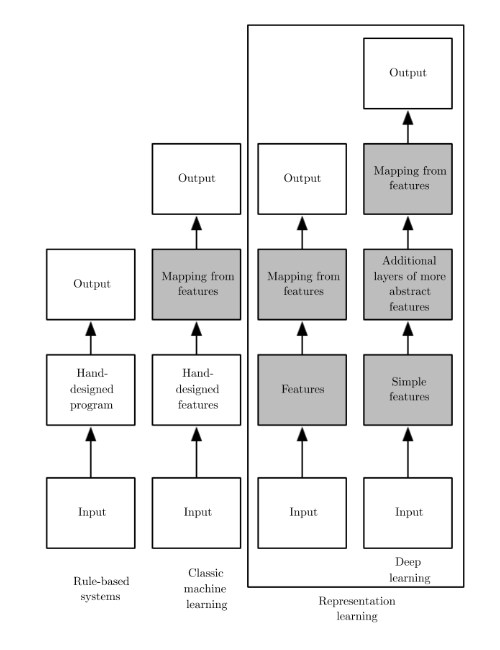
\includegraphics[width=250px]{Figures/MLintro/ml.png}
    \caption{Transition from standard programming to machine learning, highlighting components that are learned from data. Source: hyperlink: Modeling with neural networks slide 1}
    \label{fig: fromProgrammingToML}
\end{figure}

\subsection{Neural Networks and Features}

Neural networks are comprised of interconnected units known as nodes, organized into distinct layers. These layers include the input layer, which receives the initial data, and the output layer, which provides the final classification or prediction. Between these, there may be several intermediate layers. Networks with many such layers are described as deep, whereas those with few are termed shallow\cite{Sarker2021}. Each node in these networks is assigned a value between 0 and 1, and connections between nodes, known as edges, are weighted. These weights, which influence the strength of the connections, are adjustable through learning processes and are crucial for the network's ability to solve specific problems\cite{Witten2005}.

\begin{figure}
    \centering
    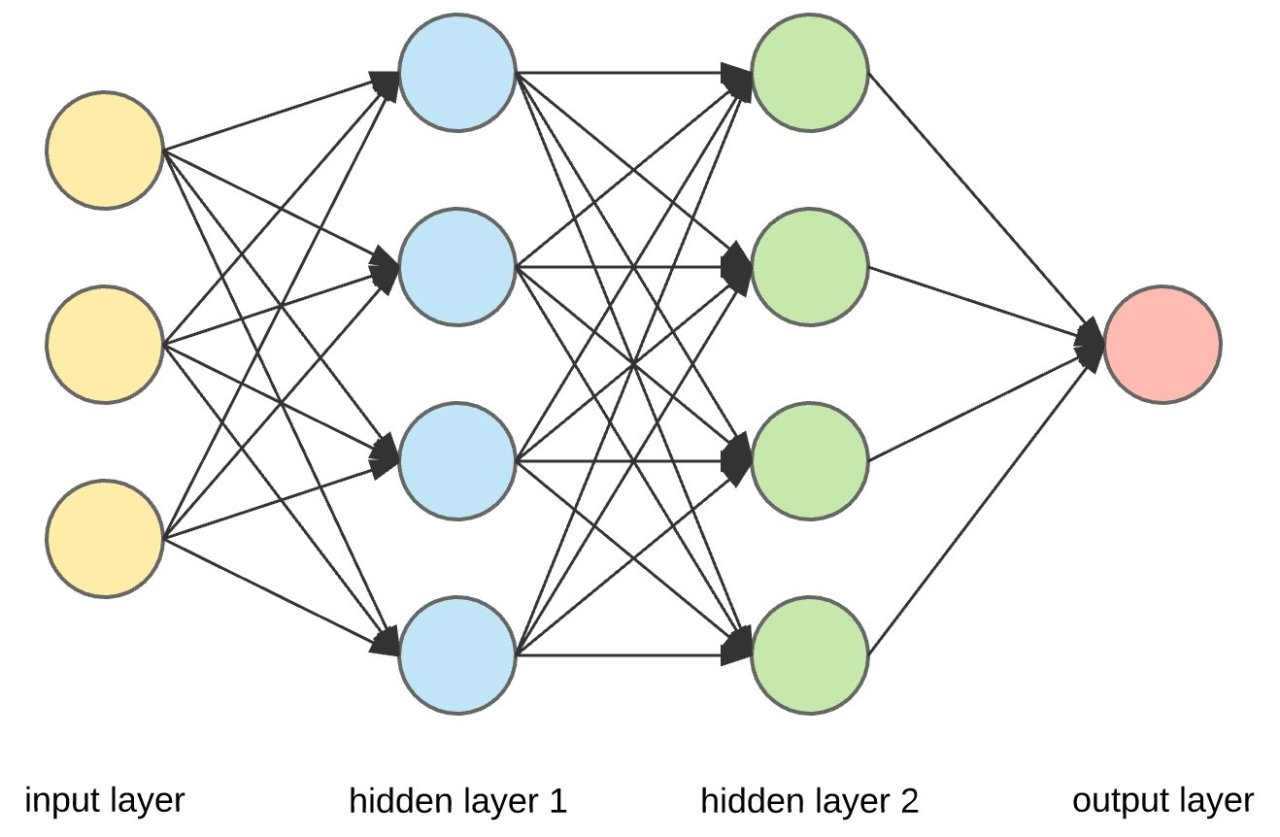
\includegraphics[width=250px]{Figures/MLintro/nn.jpg}
    \caption{Illustration of a fully connected neural network, where each node in one layer is connected to all nodes in the subsequent layer.}
    \label{fig: nn2ex}
\end{figure}

As shown in \autoref{fig: nn2ex}, the depicted neural network processes an input, such as a hand-drawn number "2." The first layer consists of nodes representing different features identifiable in various parts of the digits. Each node compares its encoded features against the input to generate a similarity score ranging from 0 to 1. Nodes not resembling any features in the input receive lower scores. Subsequent layers synthesize the information from prior layers to progressively refine the interpretation and combination of features, culminating in a final output that identifies the most likely digit represented by the input.

This example simplifies and leaves out many of the complexities inherent in neural network operation, the relevant ones of which will be addressed in detail in subsequent sections of this thesis. A critical aspect of neural networks is that their features are learned directly from data. Consequently, while a network can learn to identify common characteristics in differently drawn "2s", the specific reasons why certain features are deemed significant remain unclear. This opacity can introduce challenges, particularly in interpreting how the network makes its decisions\cite{Mohammed2016}.

\subsection{Data Integrity}
The reliability of a neural network is heavily contingent upon the data quality used during training\cite{Sarker2021}. Since weights and features within a neural network are derived from examples, poor-quality or non-representative data can significantly impair the network's performance. For instance, if all images of cats in the training set are associated with a blue sky, the model might erroneously learn to associate the presence of a blue sky with cats. This hypothetical underscores the necessity of a large and diverse dataset to ensure the neural network can generalize well from its training and function effectively in real-world conditions.

\subsection{Training a Neural Network}
Training a neural network involves adjusting the weights to predict known outcomes accurately. This process is conducted by presenting the network with numerous examples and iteratively modifying the weights based on the network's accuracy. The degree of error in the network's predictions is quantified using a metric known as the loss function. To optimize the learning process, an algorithm known as the optimizer guides the adjustments of weights, aiming to reduce the loss as efficiently as possible. Proper data partitioning is also critical to avoid overfitting, where a network might perform well on training data but poorly on unseen data. Although each of these components, loss function, optimizer, and data partitioning, are complex subjects worthy of detailed study, this thesis will provide only a concise overview, focusing on their roles in training neural networks.

\subsubsection{Loss Functions}
\label{subsubsec: loss_functions}
A loss function quantifies the discrepancy between predicted values by the network and their true values, serving as a critical component in training neural networks. The design of the loss function significantly influences learning dynamics by prioritizing certain types of errors over others\cite{Ciampiconi2023}. For instance, the Mean Absolute Error (MAE) and the Mean Squared Error (MSE) approach errors differently: MAE evaluates the absolute difference, leading to linear error sensitivity, whereas MSE squares the differences, disproportionately penalizing more significant errors. This characteristic of MSE makes it particularly effective in situations where considerable errors are unacceptable.

\[
\text{MAE} = \frac{1}{n} \sum_{i=1}^{n} |y_i - \hat{y}_i|
\]
\[
\text{MSE} = \frac{1}{n} \sum_{i=1}^{n} (y_i - \hat{y}_i)^2
\]

\subsubsection{Optimizers}
Optimizers adjust the network's weights to minimize the loss function. The process involves navigating a high-dimensional landscape defined by the loss function to find a point of minimal error, akin to finding the lowest point in a valley. A popular optimizer, ADAM, functions similarly to a ball rolling down a hill, using momentum to escape shallow local minima and gravitate towards more optimal solutions\cite{Ruder2016}. The initial position in this landscape significantly influences the effectiveness and speed of the optimization process.

\subsubsection{Data Splitting}
Informative testing of a neural network's performance requires careful data management and can be attained by splitting data into training, validation, and testing sets\cite{Joseph2020}. This strategy prevents 'data leakage,' where adjustments to the model are influenced by the test set, leading to inflated performance metrics that do not generalize to new data. The training set is used to fit the model, the validation set is used to tune model parameters, and the test set provides an unbiased model evaluation. While adjusting hyperparameters based on test set performance is not uncommon, this can lead to subtle forms of data leakage, decreasing the accuracy of the generalizability estimate. An ideal data splitting strategy, as shown in \autoref{fig: datasplitt}, minimizes these risks by ensuring that only the validation data influence model tuning. 
\begin{figure}
    \centering
    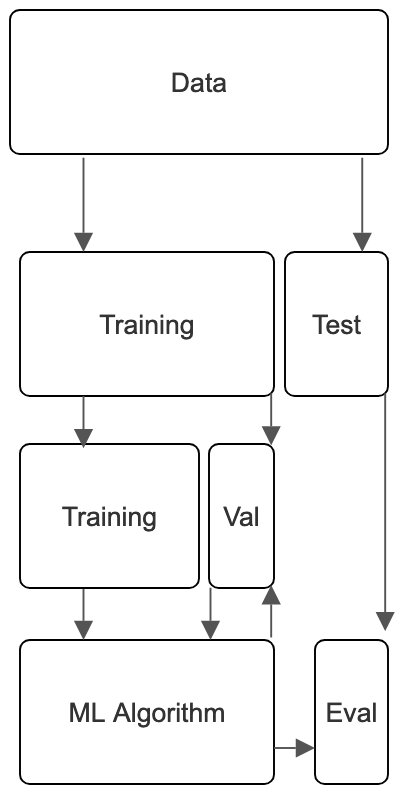
\includegraphics[width=150px]{Figures/MLintro/data_split.png}
    \caption{Idealized data splitting schema for training machine learning algorithms}
    \label{fig: datasplitt}
\end{figure}

\subsection{Overfitting}
\label{subsec: overfitting}
In machine learning, overfitting is the phenomenon where a model learns the training data too closely and subsequently fails to generalize to new, unseen data. An overfitted model can be conceptualized as one with more parameters than can be justified by the available data or that is necessary to explain it\cite{Valdenegro-Toro2022}. Mathematically, these parameters are analogous to the degree of a polynomial. The essence of overfitting is that the model inadvertently captures the noise in the data, mistaking it for the underlying data structure. This is exemplified in \autoref{fig: overfitting}.

\begin{figure}
    \centering
    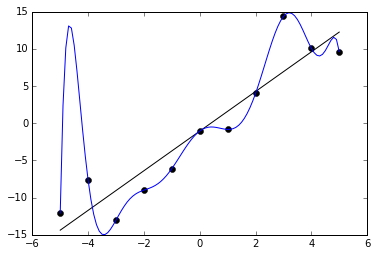
\includegraphics[width=400px]{Figures/Overfitted_Data.png}
    \caption{Demonstration of Overfitting for noisy linear data. The black dots are the data points, the black line is the linear data structure, and the blue line is the overfitted model of the data structure.}
    \label{fig: overfitting}
\end{figure}


\section{Learning paradigms}
\subsection{Supervised Learning}
Supervised learning is characterized by the use of labeled data, where each input, such as an image of a dog, is paired with a corresponding text label, in this case, "dog"\cite{Sarker2021}. The learning algorithm improves its predictions over time by adjusting weights based on the accuracy of previous predictions. This method requires a substantial volume of correctly labeled data, which can be challenging and time-consuming.

\subsection{Unsupervised Learning}
In contrast, unsupervised learning operates without labeled data, focusing instead on discovering intrinsic patterns and relationships within the dataset\cite{Sarker2021}. Not relying on predefined labels might enable the algorithm to uncover hidden structures in the data. However, this strength also introduces complexity in interpretation, as the algorithm may prioritize unexpected or non-intuitive patterns. For instance, it might cluster images based on similarities in background elements rather than distinguishing features of the subjects, such as grouping all animals photographed on grass together instead of grouping them as cats and dogs.

While this method significantly reduces the necessity for extensive labeled datasets, it demands a thorough understanding of the underlying domain to interpret and utilize the results appropriately. The potential for the algorithm to focus on irrelevant similarities poses a challenge, requiring careful analysis to ensure that the derived categorizations align with meaningful and practical insights into the data.

\section{Convolutional Neural Networks}

Due to their unique architecture, Convolutional Neural Networks (CNNs) have become a cornerstone in image classification. This architecture effectively separates feature extraction from image classification\cite{LeCun1998-CNN} as exemplified in \autoref{fig: cnn}.

\subsection{Feature Extraction Using Kernel Convolution}
CNNs utilize convolutional layers to process input images. These layers employ kernels, or small matrices, that systematically apply their weights across the image to extract features\cite{LeCun1998-CNN}. This process demonstrated in \autoref{fig: kernelconv}, involves sliding the kernel over the image and computing the dot product at each position, which emphasizes specific features like edges or textures depending on the kernel's configuration.

\begin{figure}
    \centering
    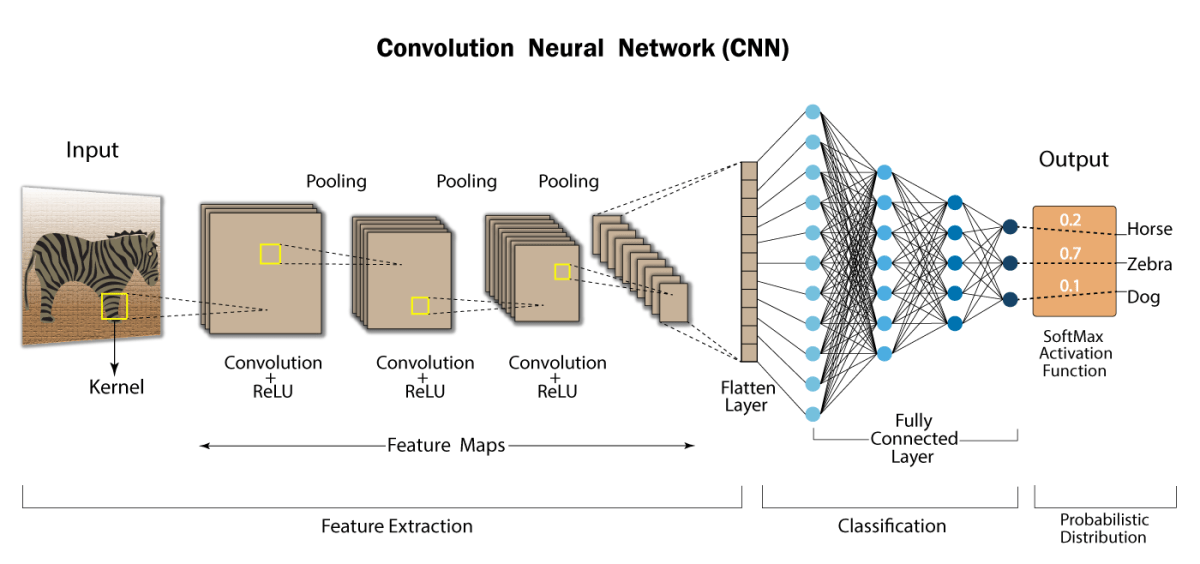
\includegraphics[width=400px]{Figures/MLintro/cnn.png}
    \caption{Visual explanation of a CNN architecture, highlighting the flow from feature extraction to classification.}
    \label{fig: cnn}
\end{figure}
\begin{figure}
    \centering
    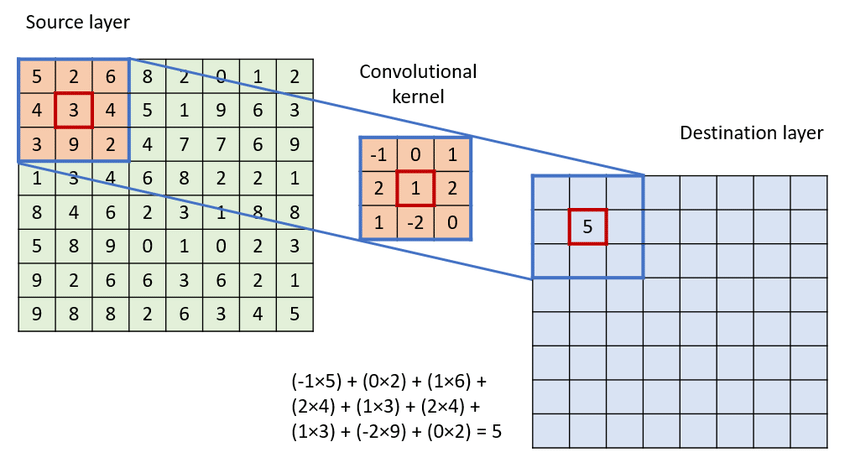
\includegraphics[width=400px]{Figures/MLintro/kernelConv.png}
    \caption{Demonstration of kernel convolution across a grayscale image to detect features.}
    \label{fig: kernelconv}
\end{figure}

For instance, a vertical line-detecting kernel might be structured as follows: 
\[
\text{Vertical Line Detecting Kernel} = 
\begin{bmatrix}
-1 & 0 & 1 \\
-1 & 0 & 1 \\
-1 & 0 & 1
\end{bmatrix}
\]
This kernel highlights vertical transitions between bright and dark regions since a vertical edge in a black-and-white image will be dark on one side and bright on the other, leading to a large number when going from dark to bright and a large negative number when going from bright to dark. This edge capturing is crucial for understanding the structure within images. By changing the structure of the kernels, different features in the image can be detected. For instance, the transpose of the Vertical Line Dection Kernel would detect horizontal lines. Crucially, the kernels are learned during the training process, not predefined, as explained here.

\subsection{Classification Using a Classic Neural Network}
After feature extraction, the subsequent layers of the CNN combine these features to form more complex representations, leading to the final classification layer. These layers are similar to traditional neural networks and integrate extracted features to effectively predict the image's content, ensuring the model generalizes well to unseen data.



\section{CNNs in the Context of EEG}
EEG signals are characterized by their complexity and non-stationary nature, presenting unique challenges in signal processing. CNNs are particularly well-suited for addressing these challenges due to their capability to handle complex data structures with the convolutional layers enabling the detection of intricate patterns within the EEG data, such as low-frequency transients, which are prominent in these signals\cite{Chen2023}.

One effective technique in enhancing CNN's performance with EEG data is the application of Continuous Wavelet Transformation (CWT). CWT transforms EEG signals into scalograms, visual representations that capture time and frequency information \cite{Arts2022}. This transformation allows CNNs to effectively localize different frequency components over time, thereby improving the detection and classification of various cognitive activities. This feature is especially beneficial given the frequent presence of artifacts and noise in EEG recordings, which can obscure critical information.

The advent of advanced CNN models such as EEGNeX marks a significant improvement in this domain \cite{demir2022eegnext}. EEGNeX has demonstrated enhanced accuracy and generalizability in classifying cognitive activities, surpassing other leading models like EEGNet\cite{Lawhern_2018}. It achieves this by effectively utilizing the spectral and temporal information inherent in EEG signals, providing a more nuanced interpretation of neural activities.

\section{Preprocessing}
Preprocessing in EEG analysis is crucial for enhancing the clarity of the signals by minimizing noise and irrelevant artifacts, which can confuse the classifier.

\subsection{IMF Selection}
\label{subsec: img_selection}
A proposed noise and artifact removal method in EEG signals involves IMF Selection, which uses the MEMD algorithm to decompose the signal into IMFs. The IMFs are then evaluated based on their Euclidean distance from the original signal, and only the \(n\) IMFs closest to the original signal are retained. This process produces a cleaner version of the original signal when recombined. An even more involved IMF selection algorithm was presented by \cite{SinghMoore2023}. There are two primary variations of the Euclidian version used in this thesis: 

\subsubsection{Individual Optimization Variation}
This variation optimizes each channel within each epoch independently, retaining only the most significant IMFs for clarity. Although this approach aims to maximize the signal cleanliness for improved classification results, it risks potential issues if IMFs across different epochs are later interchanged. Such swapping could lead to synthetic signals not representative of the underlying biological phenomena.

\subsubsection{Cross-Epoch Consistent Optimization Variation}
An alternative strategy is maintaining consistency in the IMFs selected across all epochs. This is achieved by analyzing a representative sample of epochs to determine the most important IMFs on average and retaining these for all data. This approach is less prone to errors related to IMF swapping and reduces computational complexity since it does not require optimization for every single epoch and channel. However, it risks slightly compromising the performance due to less tailored noise and artifact removal.

\subsection{Regularization}
\label{subsec: regularization}
Regularization methods are different techniques developed to reduce models' natural tendency to overfit the training data\cite{TIAN2022146}. As explained in \autoref{subsec: overfitting}, overfitted models tend to have more parameters than are necessary to understand the data. Fighting this is key in many regularization methods.

\subsubsection{L1}
\(L_1\) regularization, also known as Lasso (Least Absolute Shrinkage and Selection Operator), is a technique used to prevent overfitting by adding a penalty to the loss function. This penalty is proportional to the absolute values of the model's coefficients. The primary objective of \(L_1\) regularization is to induce sparsity in the model. Sparsity means that the model uses fewer features, as \(L_1\) regularization drives some of the coefficients to exactly zero. This effectively removes unimportant features, reducing the dimensionality and leading to better performance. The \(L_1\) can be considered analogous to the MAE form \autoref{subsubsec: loss_functions}.

\subsubsection{L2}
\(L_2\) regularization, also known as Ridge regression, is a technique used to prevent overfitting by adding a penalty to the loss function. This penalty is proportional to the square of the coefficients of the model. Unlike \(L_1\) regularization, which can drive some coefficients to zero, \(L_2\) regularization tends to shrink the coefficients towards zero but not exactly to zero. This approach helps retain all features while reducing their influence, which can lead to more stable and balanced models. The \(L_2\) can be considered analogous to the MSE form \autoref{subsubsec: loss_functions}.

\subsubsection{Dropout}
Dropout is a different kind of regularization technique designed to enhance neural networks' generalization capability. The method works by randomly deactivating a subset of neurons within the network, effectively nullifying their contribution during the training process. The proportion of neurons to be deactivated is determined by a hyperparameter known as the Dropout Rate. This rate can be fine-tuned to achieve optimal performance tailored to specific tasks. 

For instance, a Dropout Rate of 0.5 implies that 50\% of the neurons are randomly set to zero during each training iteration. The primary objective of this technique is to mitigate overfitting by preventing the network from becoming overly reliant on particular neurons. This encourages the network to develop distributed representations focusing on more robust features that are useful across different subsets of data, reducing the risk of overfitting and enhancing generalization.

\subsubsection{Early Stopping}
\label{subsec: early_stopping}
Early stopping is a regularization technique used to prevent overfitting during the training process. This method involves monitoring the model's performance on a validation set and halting the training process when the performance ceases to improve.

In practice, the training of a neural network typically involves iterating over the dataset multiple times, each iteration being called an epoch (not to be confused with epochs from neuroscience and MNE used later). During each epoch, the model's parameters are updated to minimize the loss function, improving its performance on the training data. However, if training continues for too long, the model may start to overfit.

Early stopping addresses this issue by using the validation set. After each epoch, the model's performance is evaluated on the validation set using a chosen metric, such as validation loss or accuracy. If the validation performance does not improve for a predefined number of consecutive epochs, the training process is stopped. The number of consecutive epochs it takes before stopping is called the Patience and is a tunable hyperparameter. Early stopping thus ensures that the model parameters are saved where the model performs best on the validation set, likely achieving a better generalization to unseen data.

\section{Data Augmentation}
Data augmentation is a process by which additional data is generated from existing data through modifications and transformations. These techniques often involve altering images by rotation, blurring, or other means to create variations while maintaining the core characteristics of the original data. Such artificially created data, called synthetic data, effectively enhances the dataset without needing new real-world data\cite{wang2024comprehensive}.
\subsection{Augmentation Ratio}
\label{subsec: augmentation_ratio}
The augmentation ratio is how much additional data should be added as synthetic data. A higher ratio results in more data, but the synthetic proportion also increases. The formula is: 

\begin{equation}
\text{synthetic\_data\_len} = \text{len(real\_data)} \times \text{augmentation\_ratio}
\end{equation}

Thus, a ratio of 1.0 will mean 50\% of the total data is synthetic. 

\section{Unbalanced Datasets}
\label{unbalanced_dataset_theory}
A significant challenge in supervised learning is the uneven distribution of classes within datasets. Predominant classes can bias the model to favor the majority class, undermining the model's ability to learn from less frequent classes. For instance, in a binary classifier where one class constitutes 95\% of the data, a model predicting this majority class exclusively would achieve a 95\% accuracy despite not genuinely discerning the underlying patterns distinct to each class but instead relying solely on the class distribution.

\subsection{Data Balancing Methods}
To mitigate the effects of class imbalance, several strategies have been developed\cite{10061154}: 

\subsubsection{Undersampling}
Undersampling involves randomly removing instances from the majority class to equalize the class distribution. This method directly reduces the volume of data, potentially eliminating valuable information, but it avoids creating synthetic data and duplicating existing data.

\subsubsection{Oversampling}
In contrast, oversampling increases the representation of the minority class by duplicating its instances. This method preserves valuable data from the majority class but risks overfitting, as it increases the likelihood of the model learning noise and specific patterns from the duplicated minority class examples.

\subsubsection{Synthetic Minority Oversampling Technique (SMOTE)}
SMOTE enhances dataset balance through synthetic data generation for the minority class. This technique selects a random instance \(A\) from the minority class, identifies its \(k\) nearest neighbors, chooses one neighbor \(B\), and generates a new sample \(C\) based on a point along the line segment connecting \(A\) and \(B\) in feature space. SMOTE alleviates the duplication issue prevalent in traditional oversampling but can produce ambiguous class boundaries if class distributions overlap significantly. The creation process does not account for majority class characteristics, which might lead to less effective learning in areas where classes intersect \cite{smote}.

\subsubsection{Class Weight Balancing}
Class weight balancing adjusts the impact of each class during the training process based on its representation. Classes with fewer samples are given higher relative importance, calculated using the formula: 
\[
\frac{n_{\text{samples}}}{n_{\text{classes}} \cdot \text{np.bincount}(y)}
\]
Here, \(n_{samples}\) refers to the total number of samples, \(n_{classes}\) the number of classes, and \(np.bincount(y)\) gives the number of samples in each class.
This method effectively increases the model's sensitivity to the minority class without altering the data distribution.

\subsubsection{Synthetic MEMD Minority Oversampling Technique (SMEMD-MOTE)}
SMEMD-MOTE is tailored for EEG signal datasets and uses synthetic data generation to balance classes. It involves selecting two random samples, decomposing them into their respective IMFs, swapping some of their IMFs, and recombining these to form a new, synthetic signal within the same class. This technique builds on the principles of SMOTE and is adapted to EEG data analysis's unique characteristics and requirements.


\section{Testing Model Performance}
\label{performanceMetrics}

This section outlines some metrics used to evaluate the effectiveness of machine learning binary classifiers\cite{rainio2024evaluation}.

\subsection{Accuracy}
Accuracy is the most intuitive performance measure, and it is simply a ratio of correctly predicted observations to total observations. It is useful when the target classes in the dataset are nearly balanced. Accuracy is calculated as: 
\[
\text{Accuracy} = \frac{\text{Number of correct predictions}}{\text{Total number of predictions}}
\]

\subsection{Precision}
Precision (also called positive predictive value) is the ratio of correctly predicted positive observations to the total predicted positives. It can be an essential measure in scenarios where the cost of a false positive is high.
\[
\text{Precision} = \frac{\text{True Positives}}{\text{True Positives + False Positives}}
\]

\subsection{Recall}
Recall (also known as sensitivity) is the ratio of correctly predicted positive observations to all observations belonging to the positive class. Thus, it measures how many of the objects in the positive class were labeled correctly.
\[
\text{Recall} = \frac{\text{True Positives}}{\text{True Positives + False Negatives}}
\]

\subsection{F1 Score}
The F1 Score is the weighted average of Precision and Recall. Therefore, this score takes both false positives and false negatives into account. It is beneficial when the classes are imbalanced. The F1 score is the harmonic mean of precision and recall: 
\[
\text{F1 Score} = 2 \cdot \left(\frac{\text{Precision} \cdot \text{Recall}}{\text{Precision + Recall}}\right)
\]

\subsection{AUROC}
The Area Under the Receiver Operating Characteristic curve (AUROC, sometimes AUC) represents the measure of the ability of the model to distinguish between the classes. An AUROC of 0.5 suggests no discriminative ability (chance), while 1.0 represents perfect discrimination and 0.0 is inverse discrimination. For a binary classification model (“OT” vs. “MW”), the AUROC tells you the probability that a randomly selected “OT” class member will have a higher predicted probability of being classified as “OT” than a randomly selected “MW” image.

\subsection{Kappa}
The Kappa statistic (or Cohen's Kappa) measures the prediction agreement with the true values. It is normalized by the imbalance of the classes in the data, making it more reliable when classes are unbalanced. The Kappa statistic considers random chance in the accuracy calculation, providing a more nuanced understanding of model performance.
\[
\text{Kappa} = \frac{P_o - P_e}{1 - P_e}
\]
Where \(P_o\) is the relative observed agreement among raters (i.e., accuracy), and \(P_e\) is the hypothetical probability of chance agreement.

Each metric provides unique insights into the model's performance, enabling a comprehensive evaluation beyond simple accuracy. 
